\emph{Inteligencia artificial} es definida como ``el esfuerzo por automatizar tareas intelectuales normalmente realizadas por humanos''\cite{cho18}, de este campo general se desprenden el \emph{aprendizaje maquinal} y el \emph{aprendizaje profundo}.

\begin{center}
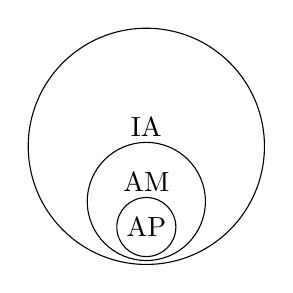
\begin{tikzpicture}
\def\AI{(0,0) circle (1.5cm)}
\def\ML{(270:.7cm) circle (.75cm)}
\def\DL{(270:1.025cm) circle (.375cm)}
\draw \AI node[above]{IA};
\draw \ML node[above]{AM};
\draw \DL node{AP};
\end{tikzpicture}
\caption{tal vez me sirva para resumir, imagen no es para producto final}
\end{center}